%-----------------------------------------------------------------------
%
%     This file is part of the Code_Saturne Kernel, element of the
%     Code_Saturne CFD tool.
%
%     Copyright (C) 1998-2008 EDF S.A., France
%
%     contact: saturne-support@edf.fr
%
%     The Code_Saturne Kernel is free software; you can redistribute it
%     and/or modify it under the terms of the GNU General Public License
%     as published by the Free Software Foundation; either version 2 of
%     the License, or (at your option) any later version.
%
%     The Code_Saturne Kernel is distributed in the hope that it will be
%     useful, but WITHOUT ANY WARRANTY; without even the implied warranty
%     of MERCHANTABILITY or FITNESS FOR A PARTICULAR PURPOSE.  See the
%     GNU General Public License for more details.
%
%     You should have received a copy of the GNU General Public License
%     along with the Code_Saturne Kernel; if not, write to the
%     Free Software Foundation, Inc.,
%     51 Franklin St, Fifth Floor,
%     Boston, MA  02110-1301  USA
%
%-----------------------------------------------------------------------
\section{General description}
%----------------


        \subsection{Objective}
%-----------------------------
The aim of this case is to train the user of \CS on an oversimplified 2D junction
including an inlet, an outlet, walls and symmetries.

        \subsection{Description of the configuration}
%-----------------------------------------------

The configuration is two-dimensional.\\
It consists of a simple junction as shown on figure \ref{figante11}.
The flow enters through a hot inlet into a cold
environment and exits as indicated on the same figure. This geometry can be
considered as a very rough approximation of the cold branch and the downcomer of
the vessel in a nuclear pressurized water reactor. The effect of temperature on
the fluid density is not taken into account in this first example.

\begin{figure}[h!]
\begin{center}
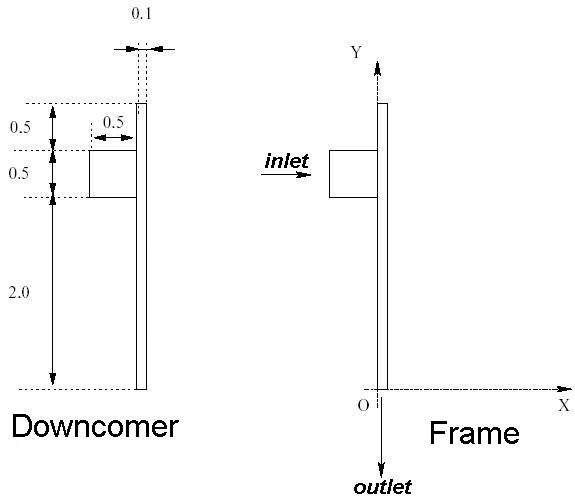
\includegraphics[width=9cm,height=8cm]{fig01}
\caption{Geometry of the downcomer}
\label{figante11}
\end{center}
\end{figure}

        \subsection{Characteristics}
%----------------------------------

Characteristics of the geometry and the flow:
\begin{center}
\begin{tabular}{|l|c|}
\hline
Height of downcomer & $H = 3.00\ m$ \\
\hline
Thickness of downcomer & $E_{d} = 0.10\ m$ \\
\hline
Diameter of the cold branch & $D_{b} = 0.50\ m$ \\
\hline
Inlet velocity of fluid & $V = 1\ m.s^{-1}$ \\
\hline
\end{tabular}\\
\end{center}

Physical characteristics of fluid:\\
The initial water temperature in the domain is equal to 20\degresC.
The inlet temperature of water in the cold branch is 300\degresC.
Water characteristics are considered constant and their values taken at
300\degresC\ and $150\times 10^{5}\ Pa$:
\begin{itemize}
        \item density: $\rho = 725.735\ kg.m^{-3}$
        \item dynamic viscosity: $\mu = 0.895\times10^{-4}\ kg.m^{-1}.s^{-1}$
        \item specific heat: $C_{p} = 5\,483\ J.kg^{-1}.\mbox{\degresC}^{-1}$
        \item Thermal Conductivity $ = 0.02495\ W.m^{-1}.K^{-1}$
\end{itemize}


        \subsection{Mesh characteristics}
%---------------------------------------

Figure \ref{figante12} shows a global view of the downcomer mesh. This
two-dimensional mesh is composed
of 700 cells, which is very small compared to those used in real
studies. This is
a deliberate choice so that tutorial calculations run fast.

\begin{figure}[h!]
\begin{center}
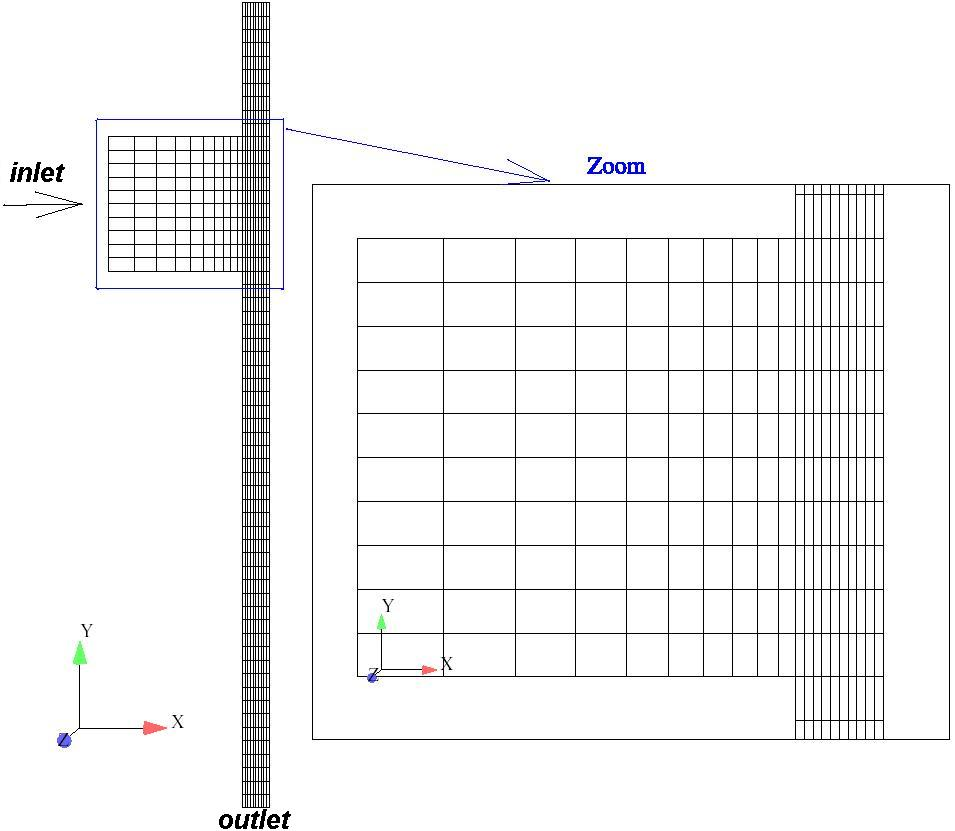
\includegraphics[width=8cm,height=7cm]{fig02}
\caption{Geometry of the downcomer}
\label{figante12}
\end{center}
\end{figure}

Note that here the case is two-dimensional but \CS always operates on three-dimensional
mesh elements (cells). The present mesh is composed of a layer of hexahedrons
created from the 2D mesh shown on figure \ref{figante12} by
extrusion (elevation) in the $Z$ direction. The virtual planes
parallel to $Oxy$ will have ``sliding'' (``symmetry'') conditions to account for
the two-dimensional character of the configuration.\\

{\bfseries Type}: structured mesh

{\bfseries Coordinates system}: cartesian, origin on the edge of the main
pipe at the outlet level, on the nozzle side (figure \ref{figante11})

{\bfseries Mesh generator used}: SIMAIL

{\bfseries Color definition}: see figure \ref{figante13}. To specifiy boundary
conditions on the boundary faces of the mesh, the latter have to be
identified. It is commonly done by assigning an integer to each of them,
characteristic of the boundary region they belong to. This integer is refered to
as "color" or "reference".

\begin{figure}[ht]
\begin{center}
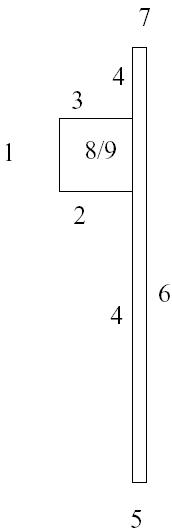
\includegraphics[width=2.5cm,height=6cm]{fig03}
\caption{Colors of the boundary faces}
\label{figante13}
\end{center}
\end{figure}


%-----------------------------------
\section{CASE 1: Basic calculation}
%-----------------------------------

        \subsection{Calculation options}
%-----------------------------------------

Most of the options used in this calculation are default options of \CS.
\begin{itemize}
\renewcommand{\labelitemi}{$\rightarrow$}
        \item Flow type: steady flow
        \item Turbulence model: $k-\epsilon$
        \item Scalar(s): 1 - temperature
        \item Physical properties: uniform and constant
\end{itemize}


        \subsection{Initial and boundary conditions}
%---------------------------------------------------

\begin{itemize}
\renewcommand{\labelitemi}{$\rightarrow$}
        \item Initialization: none (default values)
\end{itemize}


The boundary conditions are defined as follows:
\begin{itemize}
        \item {\bfseries Flow inlet}: Dirichlet condition, an inlet velocity of
$1\ m.s^{-1}$ and an inlet temperature of 300\degresC\ are imposed
        \item {\bfseries Outlet}: default values
        \item {\bfseries Walls}: default values
\end{itemize}

Figure \ref{figante13} shows the colors used for boundary conditions and
table \ref{tabante11} defines the correspondance between the colors and
the type of boundary condition to use.

Do not forget to enter the value of the hydraulic diameter, adapted to the
current inlet (used for turbulence entry conditions).\\

\begin{table}[htp]
\begin{center}
\begin{tabular}{|c|c|}
\hline
Colors & Conditions \\
\hline
1 & Inlet \\
\hline
5 & Outlet \\
\hline
2 3 4 6 7 & Wall \\
\hline
8 9 & Symmetry\\
\hline
\end{tabular}
\caption{\label{tabante11}Boundary conditions and associated references}
\end{center}
\end{table}

        \subsection{Parameters and User routines}
%------------------------------------------------

All parameters necessary to this study can be defined through the Graphical
Interface without using any user Fortran files.

\begin{center}
\begin{tabular}{|l|c|}
\hline
\multicolumn{2}{|c|}{Calculation control parameters} \\
\hline
Number of iterations & $30$ \\
\hline
Relaxation coefficient & $0.9$ \\
\hline
Output period for post-processing files& $1$ \\
\hline
\end{tabular}
\end{center}



        \subsection{Results}
%---------------------------

Figure \ref{fige1_e1} presents the results obtained at different iterations in the
calculation. They were plotted from the post-processing files, with EnSight.

\textbf{Note:} since the ``steady flow'' option has been chosen, the evolution
of the flow iteration after iteration has no physical meaning. It is merely an
indication of the rapidity of convergence towards the (physical) steady state.

\begin{figure}[h]
\parbox{0.5\textwidth}{%
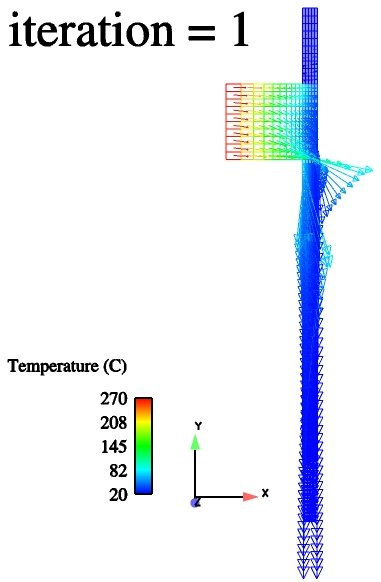
\includegraphics[width=4cm]{cas1_t_1}}
\parbox{0.5\textwidth}{%
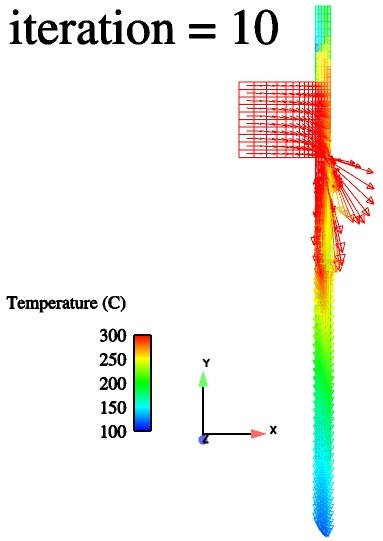
\includegraphics[width=4cm]{cas1_t_10}}
\vspace*{0.5cm}
\parbox{0.5\textwidth}{%
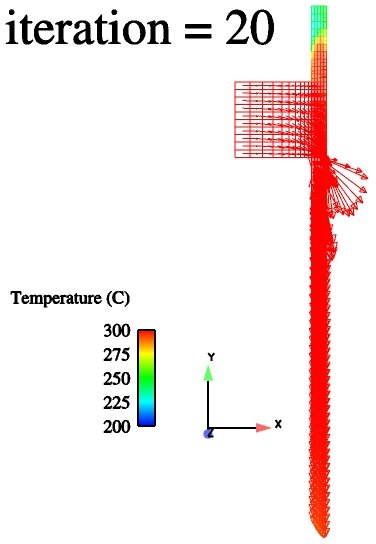
\includegraphics[width=4cm]{cas1_t_20}}
\parbox{0.5\textwidth}{%
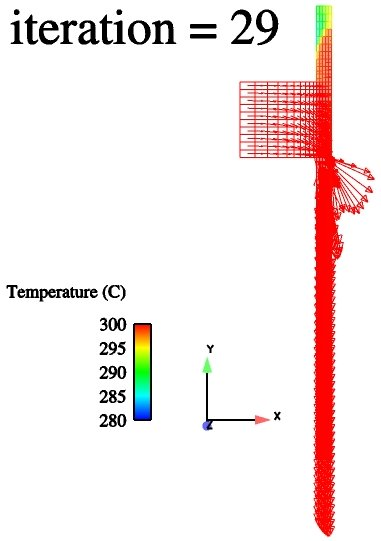
\includegraphics[width=4cm]{cas1_t_29}}
\caption{\label{fige1_e1}Water velocity field colored by temperature at different time steps}
\end{figure}


